\documentclass[a4paper, 11pt]{article}         % Paper and font size
\usepackage[english]{babel}                     % Language setting
\usepackage[style=authoryear-ibid,backend=biber]{biblatex}
\addbibresource{bibliography.bib}

% Customize your title, name, place and date here to change title, header, footer, etc.
\newcommand{\titlefirstpage}{A direct summation 3d simulation of a globular cluster}
\newcommand{\titleheaderline}{\titlefirstpage{}}
\newcommand{\authorname}{Leonardo Quiñonez}
\newcommand{\authormail}{a12411091@unet.univie.ac.at}
\newcommand{\authordate}{\today{}}
\newcommand{\authorplace}{Wien}

% Set margins
\usepackage[top=2.5cm,bottom=2.5cm,left=2cm,right=2cm,marginparwidth=1.75cm]{geometry}

% Load useful packages
\usepackage{graphicx}                           % Graphics
\usepackage{amsmath}                            % Math
\usepackage{xcolor}                             % Link color
\usepackage{subcaption}
\definecolor{custom-blue}{RGB}{0,99,166} 
\usepackage{hyperref}
\hypersetup{colorlinks=true, allcolors=custom-blue}

\usepackage{fancyhdr}                           % Load header, footer package
\usepackage{csquotes}                           % textcite, parencite, etc.
\usepackage{lastpage}                           % Footer note
\usepackage{lipsum}                             % For dummy text
\usepackage[                                    % \say for quotation marks
                                                % configure to use german-style quotes
left = \glqq,%
right = \grqq,%
leftsub = \glq,%
rightsub = \grq%
]{dirtytalk}

\pagestyle{myheadings}                          % Own header
\pagestyle{fancy}                               % Own style
\fancyhf{}                                      % Clear header, footer

\setlength{\headheight}{30pt}                   % Set header hight
\renewcommand{\headrulewidth}{0.5pt}            % Top line
\renewcommand{\footrulewidth}{0.5pt}            % Bottom line

\fancyhead[L]{
\includegraphics[width=3cm]{univienna-logo.eps}} % Header left
\fancyhead[C]{}                                                % Header center
\fancyhead[R]{\titleheaderline}                                % Header right
\fancyfoot[L]{\authorname}                                     % Footer left
\fancyfoot[C]{                                                 % Footer center
  \thepage
  % uncomment next line also include the total page count
  % /\pageref{LastPage}
}
\fancyfoot[R]{test}                                   % Footer right

%%% Begin document %%%
\begin{document}

\begin{figure}                                  % Include Logo
\flushleft

\includegraphics[width=0.4\textwidth]{univienna-logo.eps}
\end{figure}

% Set title, author, date
\title{\titlefirstpage{} \\ \large Focus project for Methods of Computational Astrophysics}

\author{\authorname{} - \authormail{}}
\date{\authordate, \authorplace}

\maketitle                                      % Include contents
%\tableofcontents

\section{State the problem}                              % Example sections, subsections

The N-body problem is a great test bed for computational methods,
multiple different techniques have been developed to tackle it, some of which were explored during the course. \parencite{Hahn2025classnotes}

The goal of this focus project is to do a direct summation 3d simulation of a globular cluster. 
Starting from a Plummer Model for the globular cluster, a leapfrog integrator would use efficient computations
of the accelerations of each body to make a 3d simulation.

Using constant equal masses and dimensionless units the equations to model the acceleration are described by:

\begin{subequations}
\begin{align}
    a(X) &= \sum_{\substack{j=1 \\ j \ne i}}^{N} \frac{\mathbf{X}_i - \mathbf{X}_j}{\|\mathbf{X}_i - \mathbf{X}_j\|^3} \label{eq:motion_b}
\end{align}
\end{subequations}

A first version of the project would be to make the simulation using the direct summation approach which has a complexity of \( \mathcal{O}(N^2) \) for \( N \) particles.
Using the different libraries we will attempt to find an efficient parallelized implementation of the direct summation.
This would be called by a leapfrog integration used to evolve the system and make a 3D simulation.


\section{Approach}                              % Example sections, subsections
The project would have the following steps:
\begin{enumerate}
    \item Efficient Direct Summation
    \item Time Integration
    \item 3D Simulation
    \item Initial Conditions
\end{enumerate}


\paragraph{Efficient Direct Summation:}
We will compare different implementations for the computation of the accelerations of N bodies.
We will focus on testing their perfomance on high number of bodies.

\begin{itemize}
    \item Python loops
    \item Vectorized Numpy
    \item Numba (Loops)
    \item Numba (Parallel)
    \item Jax (CPU)
\end{itemize}

Jax will only be tested on the CPU since the hardware available has no N-Vidia GPU.

\paragraph{Time Integration:}
A leapfrog method is chosen for its simplicity but also energy conservation properties.
The Drift Kick Drift approach is selected to simplify the implementation and have only one acceleration calculation per time step.


\paragraph{3D simulation:}
A simple as possible 3d simulation would be attempted, a search on libraries that allow the animation would be done.

\paragraph{Initial Conditions:}
The Plummer model used during the class exercises is selected for the initial conditions.


\section{Results}

\subsection{Efficient Direct Summation}
\subsubsection{Taichi}
Originally the plan was to compare the implementations described in the approach section, but when searching for 3D animation libraries the 
Taichi Lang library\footnote{Taichi Lang is a ``domain-specific language embedded in Python'' but for practical purposes it is installed any other library.  https://www.taichi-lang.org/}
 was found. It allows the usage of Vulkan\footnote{Vulkan Wikipedia Entry: https://en.wikipedia.org/wiki/Vulkan} to access the Intel integrated GPU.
The perfomance this allows for the 3D simulation and the Acceleration calculation is considerable, so it was additionally included in the comparison. 

\subsubsection{Performance Comparison}
In order to compare the perfomance of the different methods we increase the number of stars exponentially until the time to perform a single acceleration computation 
exceeds 10s. In order to account for compilation time of jit, each implementation is run three times and the median is calculated.
During this process multiple OOM(Out of Memory) errors were discovered.
This prompted to the addition of a memory usage limit of 1GB as well, to accomplish this the process data is extracted from the operating system 
every tenth of a second, this means processes with short duration times would have unreliable calculation. Even with this inaccuracy this proved
enough to avoid the OOM errors and see a full picture of all implementations performances.

Figure \ref{fig:time} shows the time comparison of the different implementations. As expected they show a polynomial complexity with exception of Taichi.
This probably is due to the use of GPU which creates a minimum time higher than CPU based alternatives, but more tests would be needed to understand this properly.
In general Jax and Taichi show the best performance, but Taichi managed to calculate one order of magnitude of stars more. 
It is important to note that Taichi and Jax are only using 32 bits to allow for a fair comparison. Given that the available GPU can't handle 64 bits.


Figure \ref{fig:space} shows the space comparison highlighting the interesting details. The numpy implementation which aimed to be a pure vectorized attempt
calculates the distance of all bodies with each other, making an NxN matrix which explains the absurd memory consumption.
Curiosly enough Jax using \texttt{vmap} presents a similar memory issue\footnote{Vmap Memory Usage Considerations: https://apxml.com/courses/getting-started-with-jax/chapter-4-automatic-vectorization-vmap/vmap-performance}.
It seems to be the case that the current implementation requires as intermediate memory the vector of distances for each star, which again reaches 
what appears to be a NxN memory footprint.
An improved implementation with Jax's \texttt{lax.map} gave better results as shown in the graph, but the additional effects of the change are yet to be understood.
\texttt{lax.map} allows to set a batch size, the small tests on this increased progressively the memory usage without a visible impact on performance.


\begin{figure}
\centering
\begin{subfigure}{.5\textwidth}
  \centering
  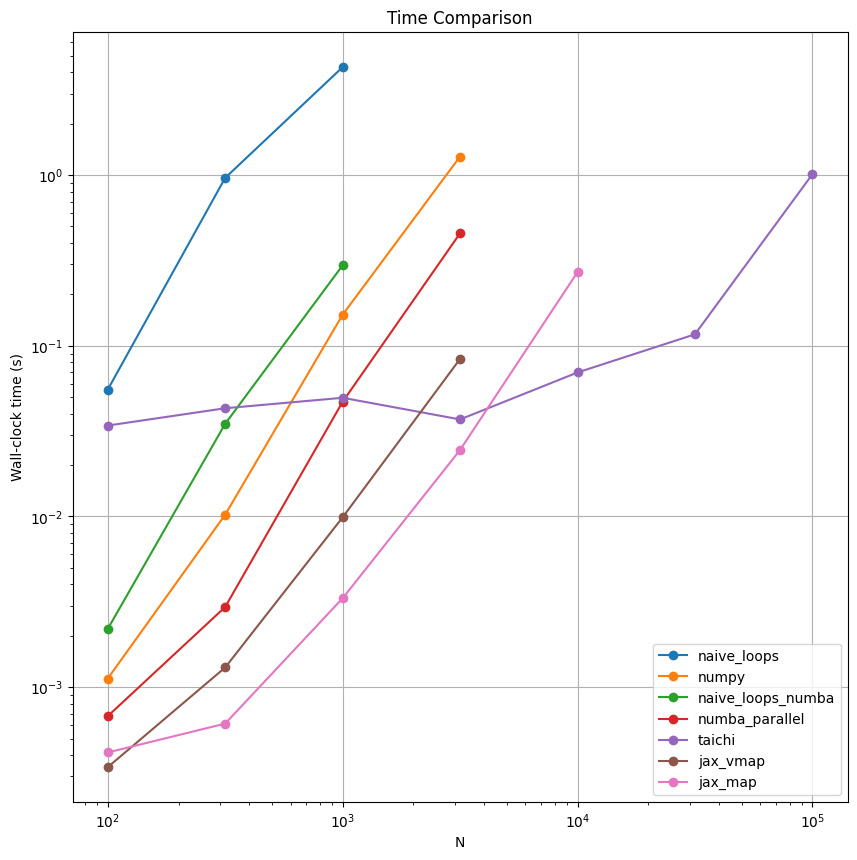
\includegraphics[width=\linewidth]{images/time_comp2}
  \caption{Time Comparison}
  \label{fig:time}
\end{subfigure}%
\begin{subfigure}{.5\textwidth}
  \centering
  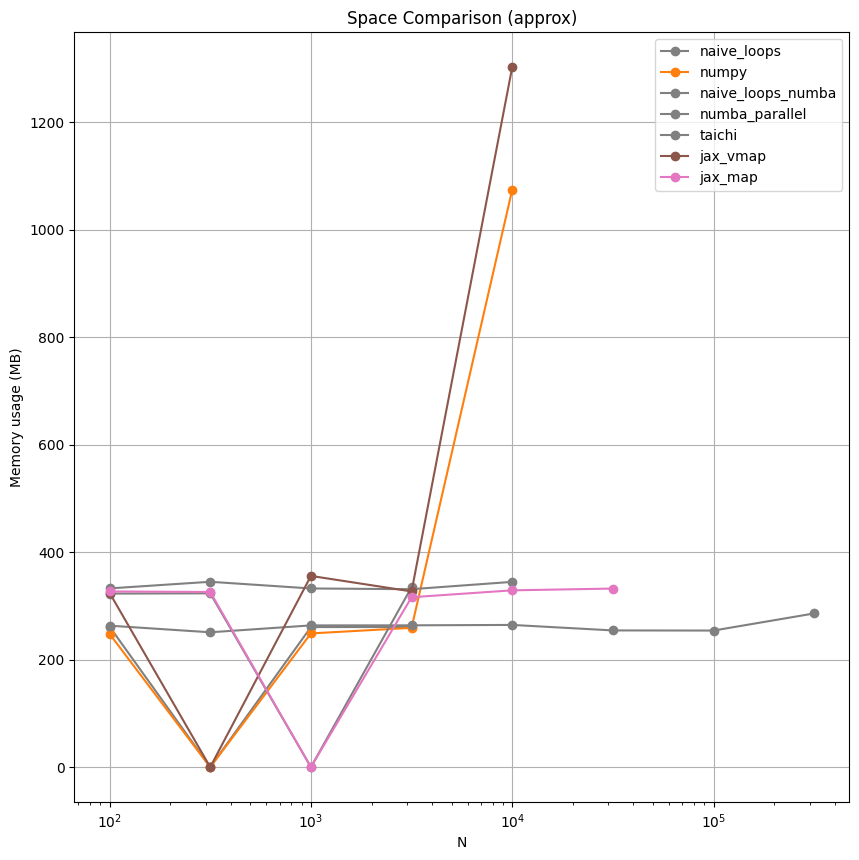
\includegraphics[width=\linewidth]{images/space_comp2}
  \caption{Space Comparison}
  \label{fig:space}
\end{subfigure}
\caption{Time and Space comparison capped to 10s and 1GB}
\label{fig:test}
\end{figure}


\subsection{3D simulation}
As 

\section{Discussion}

\section{Future}
Test with an Nvidia gpu to compare Jax performance with Taichi on equal grounds.
Implement a hierarchical method to reduce time complexity
Do a measurement of the energy of the system and maybe implement a better integration given the results.
It would be interesting as well to see the simulation works under a spectral method that allows higher number of bodies.


\subsection{Tabellen}                           % Example tables

\begin{center}
\begin{tabular}{ |c|c|c| } 
    \hline
    Cell 1 & Cell 2 & Cell 3 \\ 
    Cell 4 & Cell 5 & Cell 6 \\ 
    Cell 7 & Cell 8 & Cell 9 \\ 
    \hline
\end{tabular}
\end{center}



\printbibliography[heading=bibintoc]

%%% End document %%%
\end{document}